\documentclass[]{article}

\usepackage{graphicx}
\usepackage{url}
\usepackage{hyperref}

%opening
\title{Guided Research: Measuring and Evaluating Impact of Ray Sorting Algorithms on Coherency of SIMDs in Voxel-Based Path Tracers}
\date{April 15, 2014}

\begin{document}

\maketitle

%\begin{center}
\begin{description}
	\centering
	\item[] \textbf{Supervisor}: Prof.Dr. Ruediger Westermann
	\item[] \textbf{Advisor}: Matthaeus G. Chajdas
\end{description}
	
	
%\end{center}


\begin{abstract}

Ray-traced global illumination (GI) algorithms are becoming widespread in real-time applications and computer video games. Path tracing is a common rendering technique to render images with global illumination effect. Low performance of these algorithms, makes their usage limited. To speed up these algorithms, some acceleration hierarchy like kd-tree, BSP-tree, etc. is used. Typically, BVH-Trees are used to accelerate path-tracing algorithms. Recently, these algorithms are run in real time on CPUs and GPUs but the ray coherency after the first bounce becomes too low; As CPUs and GPUs use wide SIMD units, gaining high coherency on these units is very important. A coherency improvement mechanism can be used to restore the ray coherency. In this paper we are going to investigate the impact of ray sorting on execution coherency of processor’s SIMD units. Our measurements show that execution coherency is increased by sorting the secondary rays but the improvements in coherency values are not as much as we expected and was presented by other papers. The scenes which are rendered in our approach are voxelized and stored in Boundary Volume Hierarchy (BVH) acceleration hierarchy. Furthermore, the voxel-based path-tracer is used as global illumination technique.\newline{}

Implemented using \textbf{C++}.\newline{}

More information can be found on:\

\href{https://mmostajab.com/projects/}{https://mmostajab.com/projects/}\newline{}

\end{abstract}

\begin{description}
	\item[] 
	\item[] 
\end{description}


\begin{figure}[ht!]
	\centering
	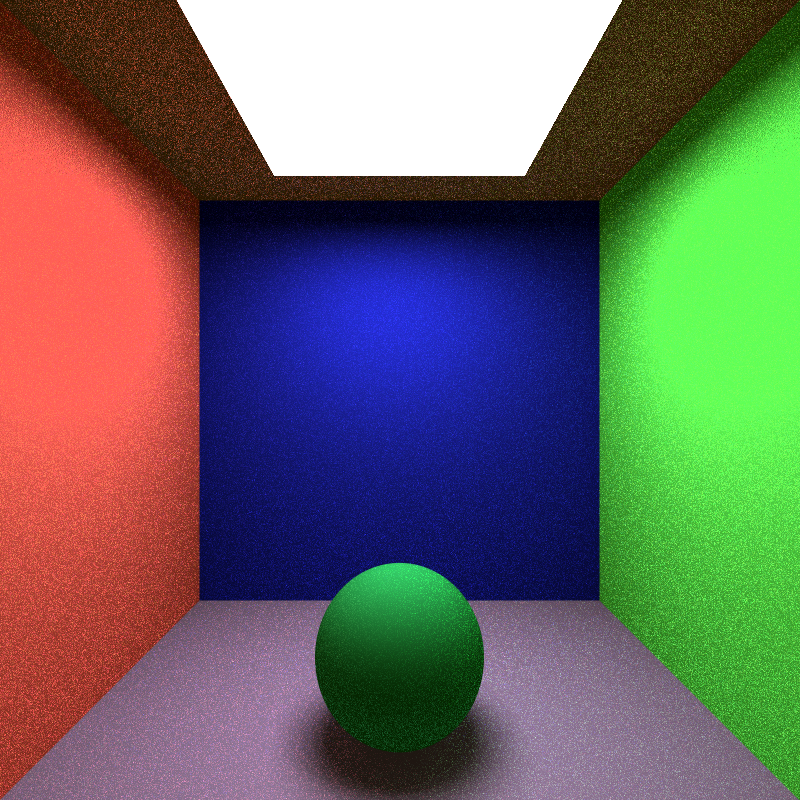
\includegraphics[width=0.45\linewidth]{gr_result2.png}		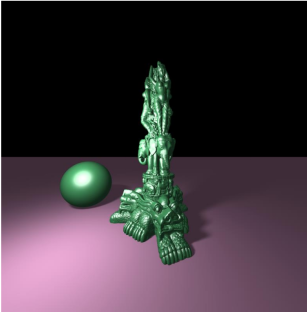
\includegraphics[width=0.45\linewidth]{gr_result.png}
	\caption{Two screenshots of output images from path-tracing Cornell box and pillar models. Both models are generated using path-tracer which I implemented from scratch in presence of an area light into the scene.}
	\label{fig:boat1}
\end{figure}


\begin{figure}[ht!]
	\centering
	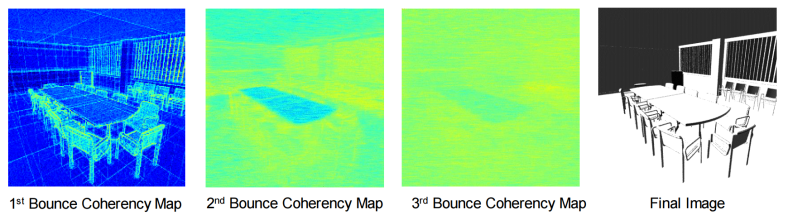
\includegraphics[width=\linewidth]{gr_compare.png}
	\caption{Coherency visualization of conference room in first, second and third bounce of the rays when rays are sorted by direction in the beginning of each bounce. The Image is rendered in 400x400 and 4 samples per pixel is used (simulated SIMD width is 16).}
	\label{fig:boat1}
\end{figure}

\end{document}
